\documentclass[a4paper,11pt]{article}

\title{Solutions to unfolding distributions}
\author{Markus Klute}
\date{\today}


\usepackage[english]{babel}
%FloatBarrier
\usepackage{placeins}
%H
\usepackage{float}
\usepackage{amsmath,amssymb,amsfonts}
\usepackage{graphicx}
\usepackage{amsmath}
\usepackage[pdftex,hyperfootnotes=false,pdfpagelabels,pagebackref]{hyperref}

% to make a analitical index/glossaries
%\usepackage[acronym,xindy,nonumberlist]{glossaries}
\usepackage[acronym,nonumberlist]{glossaries}
%\usepackage{makeidx}
\makeglossaries
%\makeindex

\usepackage{booktabs}

%caption
%\usepackage[font=small,format=plain,labelfont=bf,margin=0.05\columnwidth]{caption}
\usepackage[font=small,format=plain,labelfont=bf,margin=0.05\columnwidth]{caption}


%%%% DEFINE COMMANDS %%%%%%%%%%%
\newcommand{\meas} {\ensuremath \vec{y}}
\newcommand{\truth}{\ensuremath \vec{x}_\textup{T}}
\newcommand{\resp} {\ensuremath \mathbf{R}}
\newcommand{\back} {\ensuremath \vec{b}}

\newcommand{\respt}{\ensuremath \mathbf{\tilde{R}}}
\newcommand{\strength}{\ensuremath \vec{\mu} } 

\newcommand{\mc}{\ensuremath \vec{x}_\textup{MC}}
%% I version
\newcommand{\truthI}[1]{\ensuremath x^\textup{T}_{#1}}
\newcommand{\strengthI}[1]{\ensuremath \mu_{#1} }
\newcommand{\mcI}[1]{\ensuremath x^\textup{MC}_{#1}}
\newcommand{\respI}[2]{\ensuremath R_{#1,#2} }
\newcommand{\resptI}[2]{\ensuremath \tilde{R}_{#1,#2} }

%% FIG 
\newcommand{\Left}{\mbox{(Left)}}
\newcommand{\Right}{\mbox{(Right)}}

%%%  Draft
\newcommand{\fixme}[1]{ \mbox{\bf{FIXME:} \it{#1}} } 


\newacronym{MC}{MC}{Monte Carlo}
\newacronym{BLUE}{BLUE}{best linear unbiased estimator}
\newacronym{ML}{ML}{maximum likelihood}
\newacronym{SVD}{SVD}{singular value decomposition}



\begin{document}
\maketitle

\section{Understanding unfolding}

The Unfolded spectra can be found using, eg, RooUnfold:
\begin{verbatim}
ROOT.gSystem.Load("${HOME}/Downloads/RooUnfold-1.1.1/libRooUnfold.so")
##  prepare the response matrix
# assume a flat prior, no eff, no bkg
R = ROOT.RooUnfoldResponse(None,None,resp)
u = ROOT.RooUnfoldInvert(R,reco)
u.SetName("unfolder1")
h = u.Hreco(ROOT.RooUnfold.kNone) 
h.SetName("unfold")

## for meaningful errors
fluct=1.0
for j in range(0,reco.GetNbinsX() ):
	reco_fluct.SetBinError(j+1,fluct)

u2 = ROOT.RooUnfoldInvert(R,reco_fluct)
u2.SetName("unfolder2")
u2.SetNToys(1000)
h2 = u2.Hreco( ROOT.RooUnfold.kCovToy) ##  error propagation down with toys
h2.SetName("unfold2")

\end{verbatim}

The result is shown in figure~\ref{fig:sol1}: the unfolded distribution with no-fluctuations should be by-construction identical to the one used for generating it; 
small differences may be due to the numeric precision of the floating point representation inside a computer, that act as a fluctuation smearing. 
The one that had fluctuations inside, nevertheless is the \gls{ML} estimator and therefore the \gls{BLUE}, has a very huge variance.

\begin{figure}[H]
	\centering
	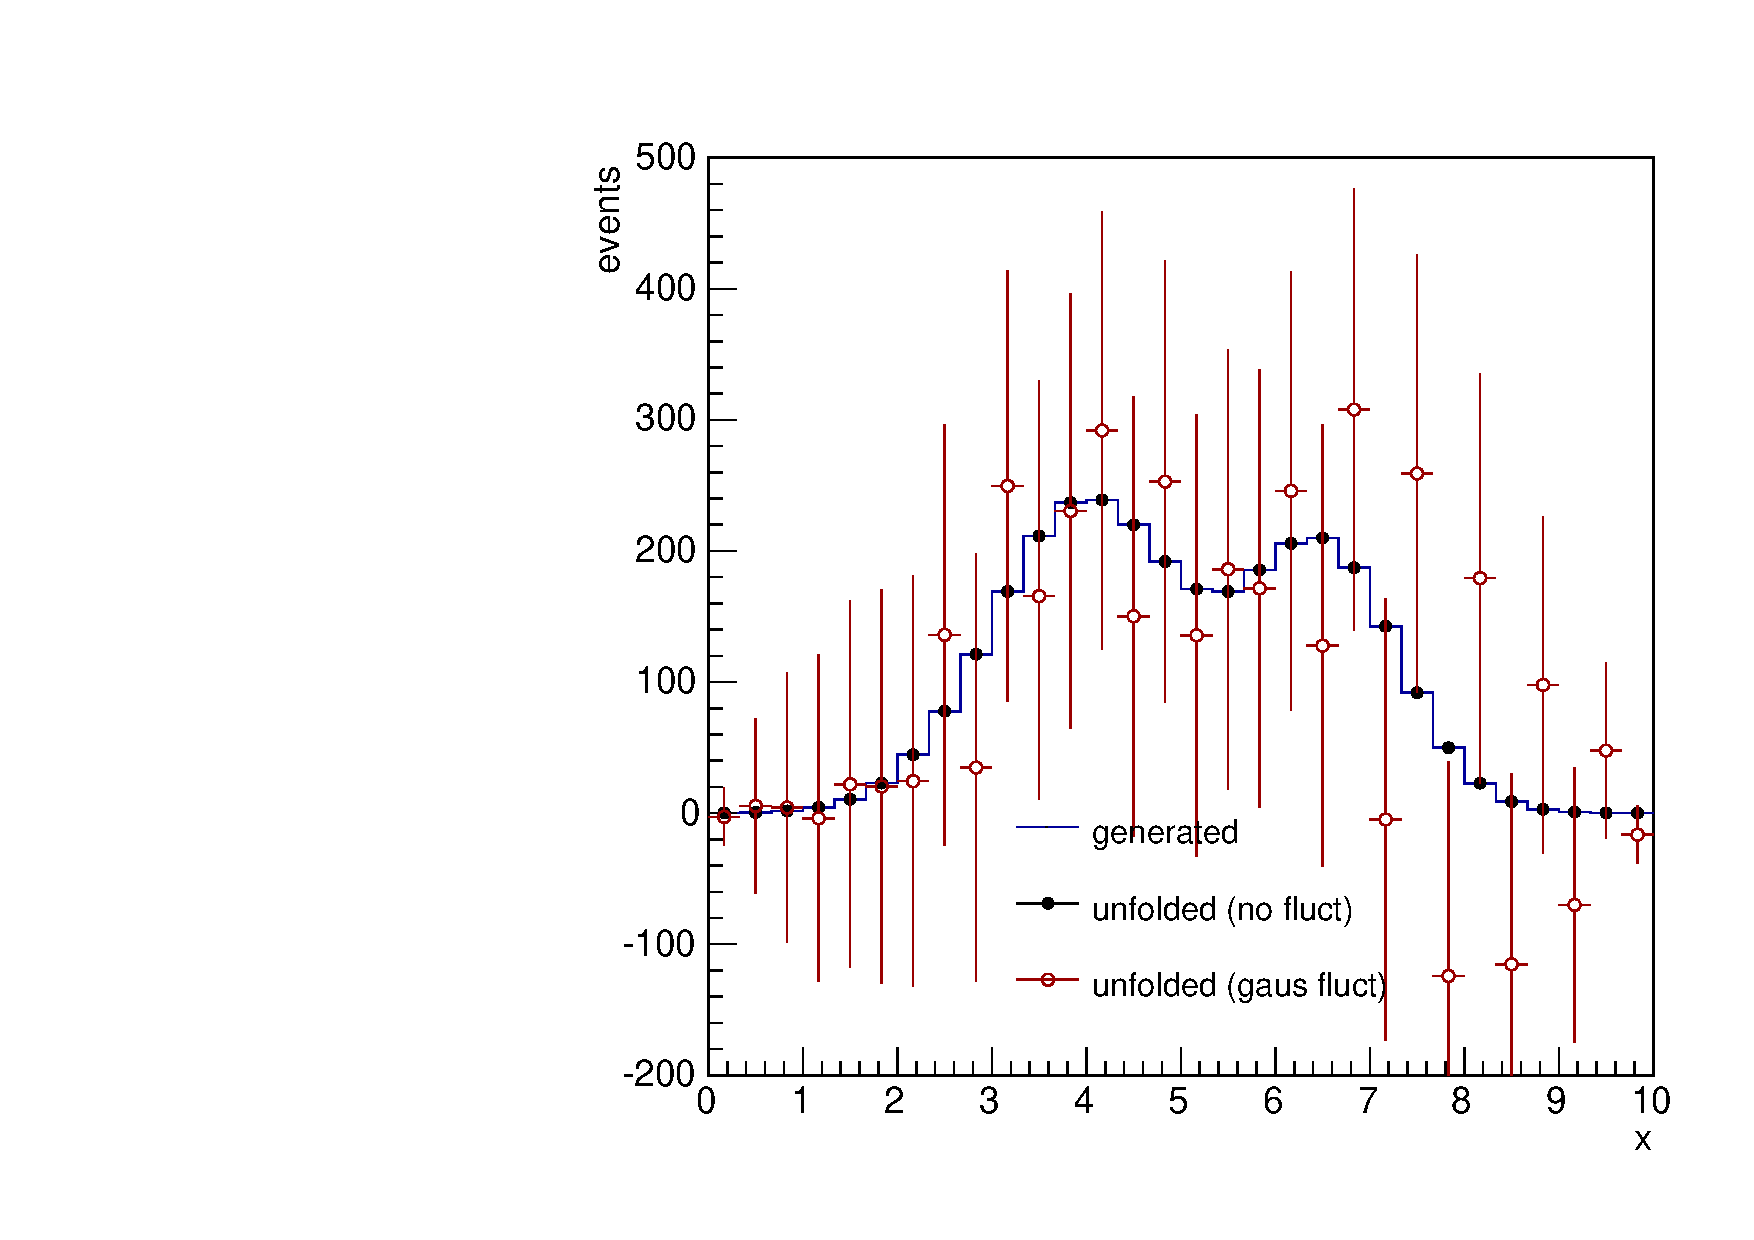
\includegraphics[width=0.618\textwidth]{figs/gen-unfold.pdf}
	\caption{ \label{fig:sol1} The two unfolded distribution compared with the one used to generate them.}
\end{figure}

\FloatBarrier
\section{Regularized unfolding}
Regularization techniques are used to cure the high variance of the distribution, introducing an ad hoc bias. 

We start studying regularization to see the effect that it has on the distributions:
\begin{figure}[H]
	\centering
	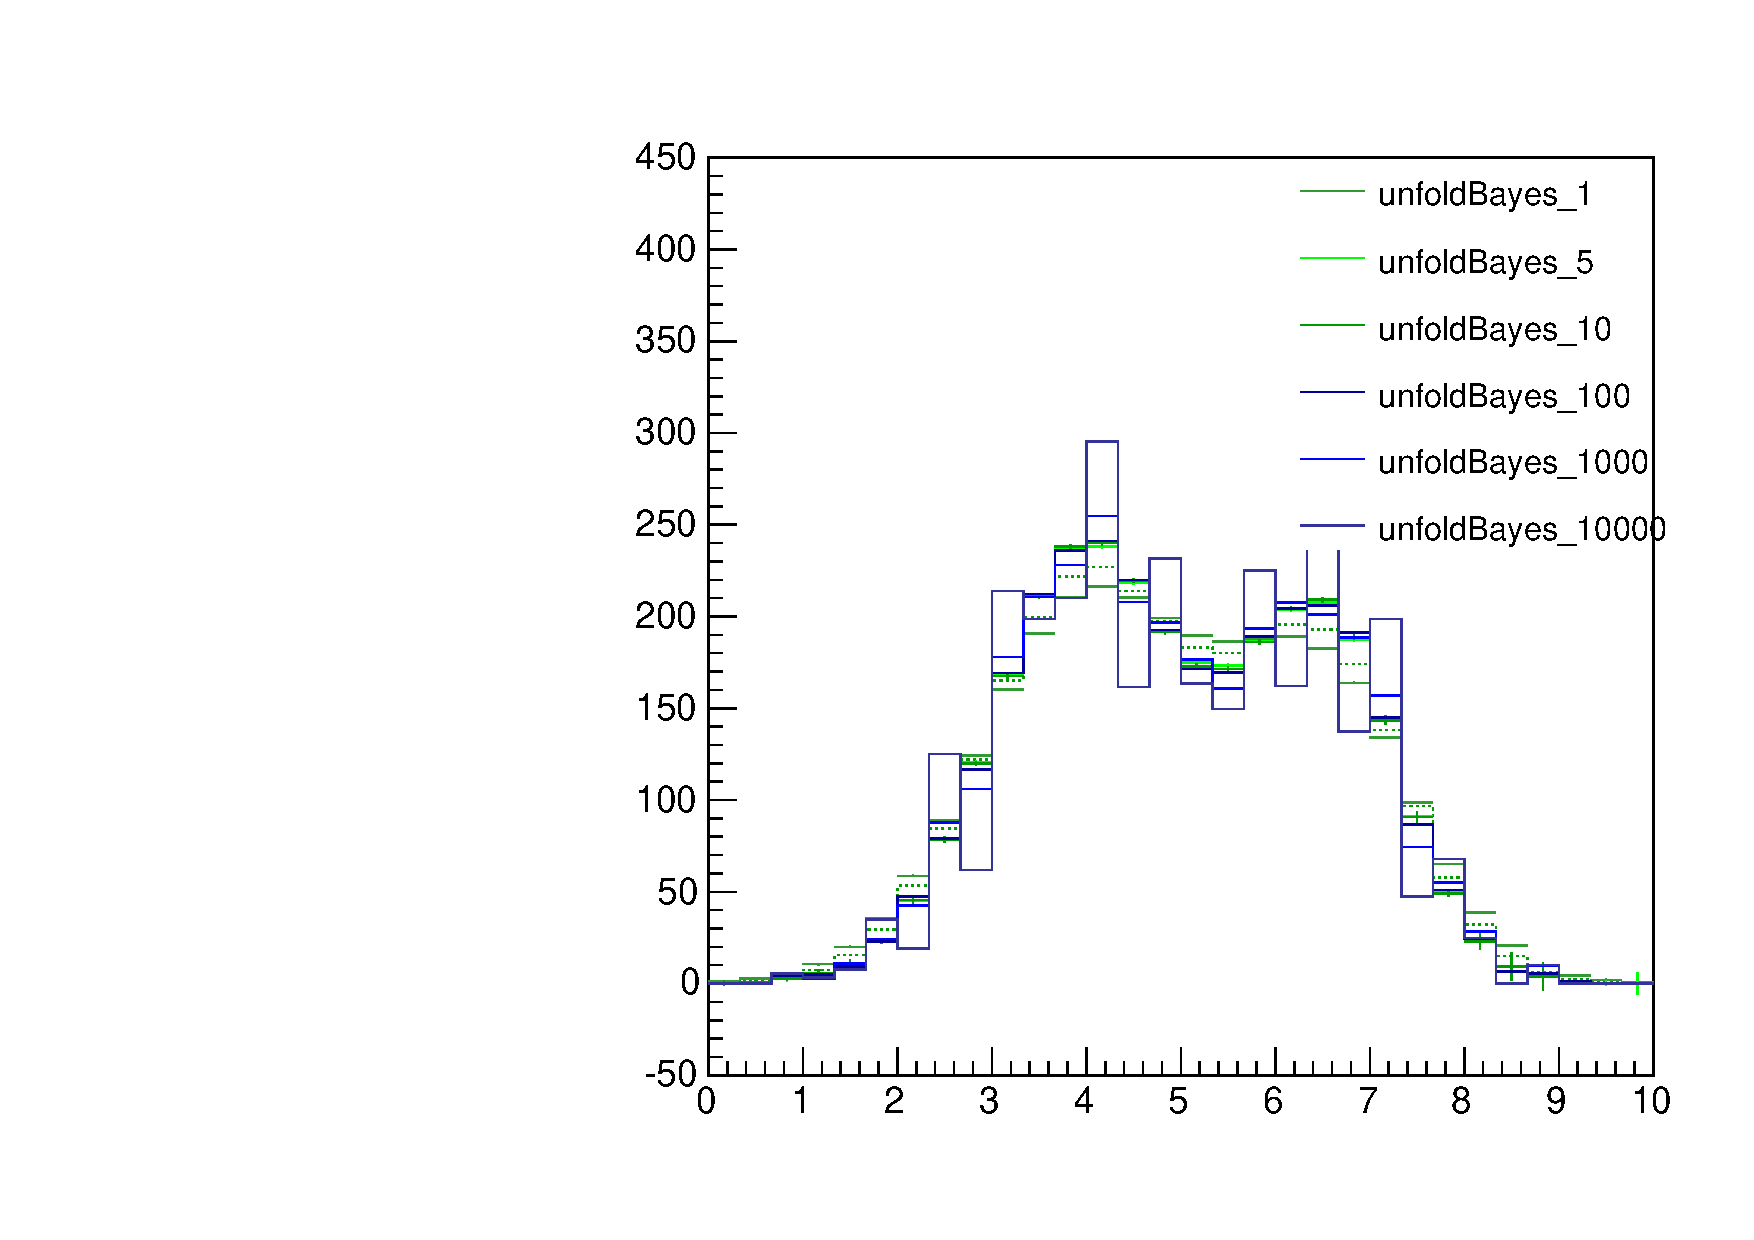
\includegraphics[width=0.49\textwidth]{figs/unfold-bayes-reg.pdf}
	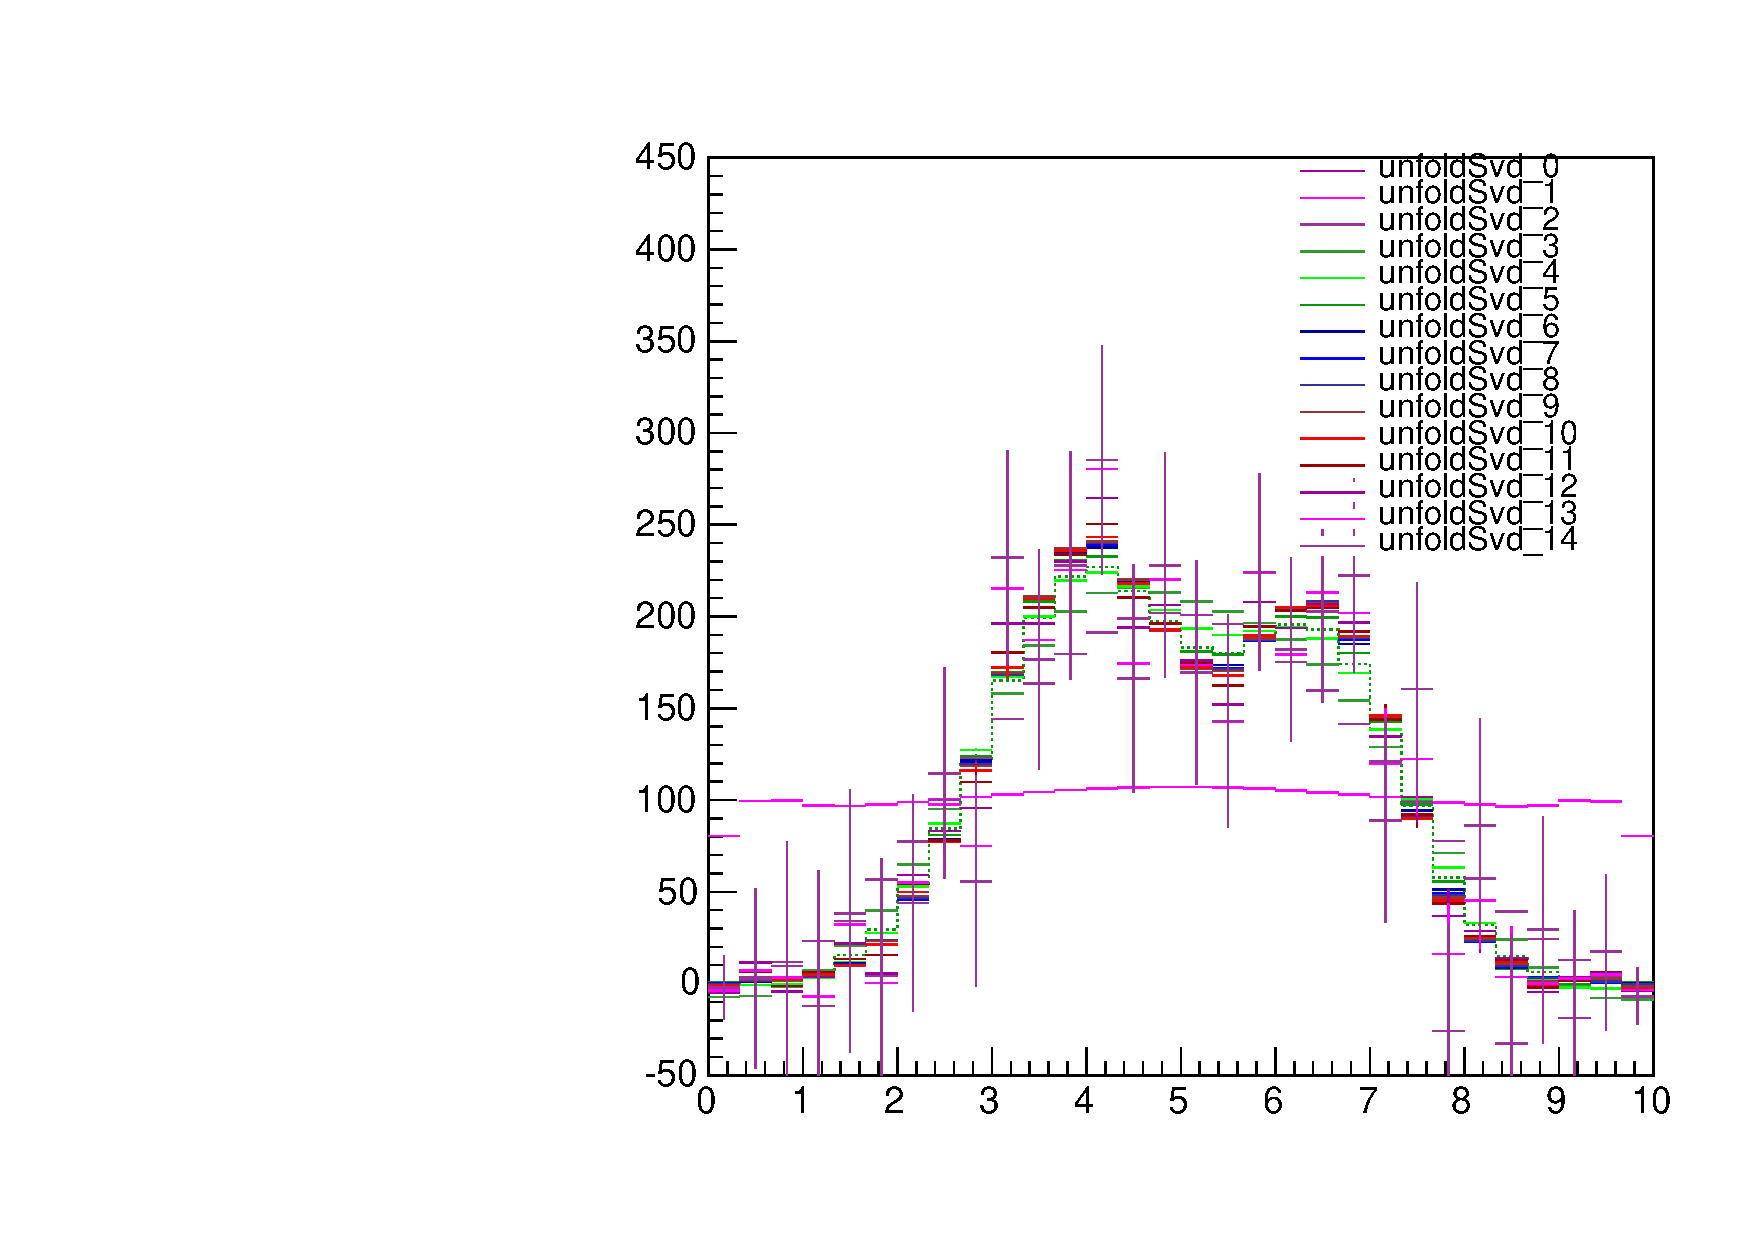
\includegraphics[width=0.49\textwidth]{figs/unfold-svd-reg.pdf}
	\caption{ \label{fig:sol:reg} The unfolded distribution for different regularization parameters. On the left, the iterative unfolding, on the right the Tikhonov regularization. }
\end{figure}

For the iterative method based on Bayes' theorem the regularization is given by the number of iteration; the less iterations the closer the unfolded distribution to the prior we choose, usually obtained from \gls{MC}. The method will converge to the \gls{ML} solution with the increasing number of iterations.
For the \gls{SVD} implementation of the Tikhonov regularization, the regularization is given by the number of singular values used in the inversion. The less singular values, the more the distribution is regularized. Using ``all'' the singular values we get close the \gls{ML} solution.

The regularization parameter is a \emph{choice} to make. 
There is no right and wrong value, but some wanted features are:
\begin{itemize}
	\item stability of the regularization with respect to the chosen regularization parameter.
	\item for the \gls{SVD}-method look at the $d_i$ distribution; in this case it shows that after $~10$ the distribution is random.
	\item error estimation after the unfolding should not be smaller than the one before it.
	\item use different predictions (if available) to evaluate possible biases.
\end{itemize}

\begin{figure}[H]
	\centering
	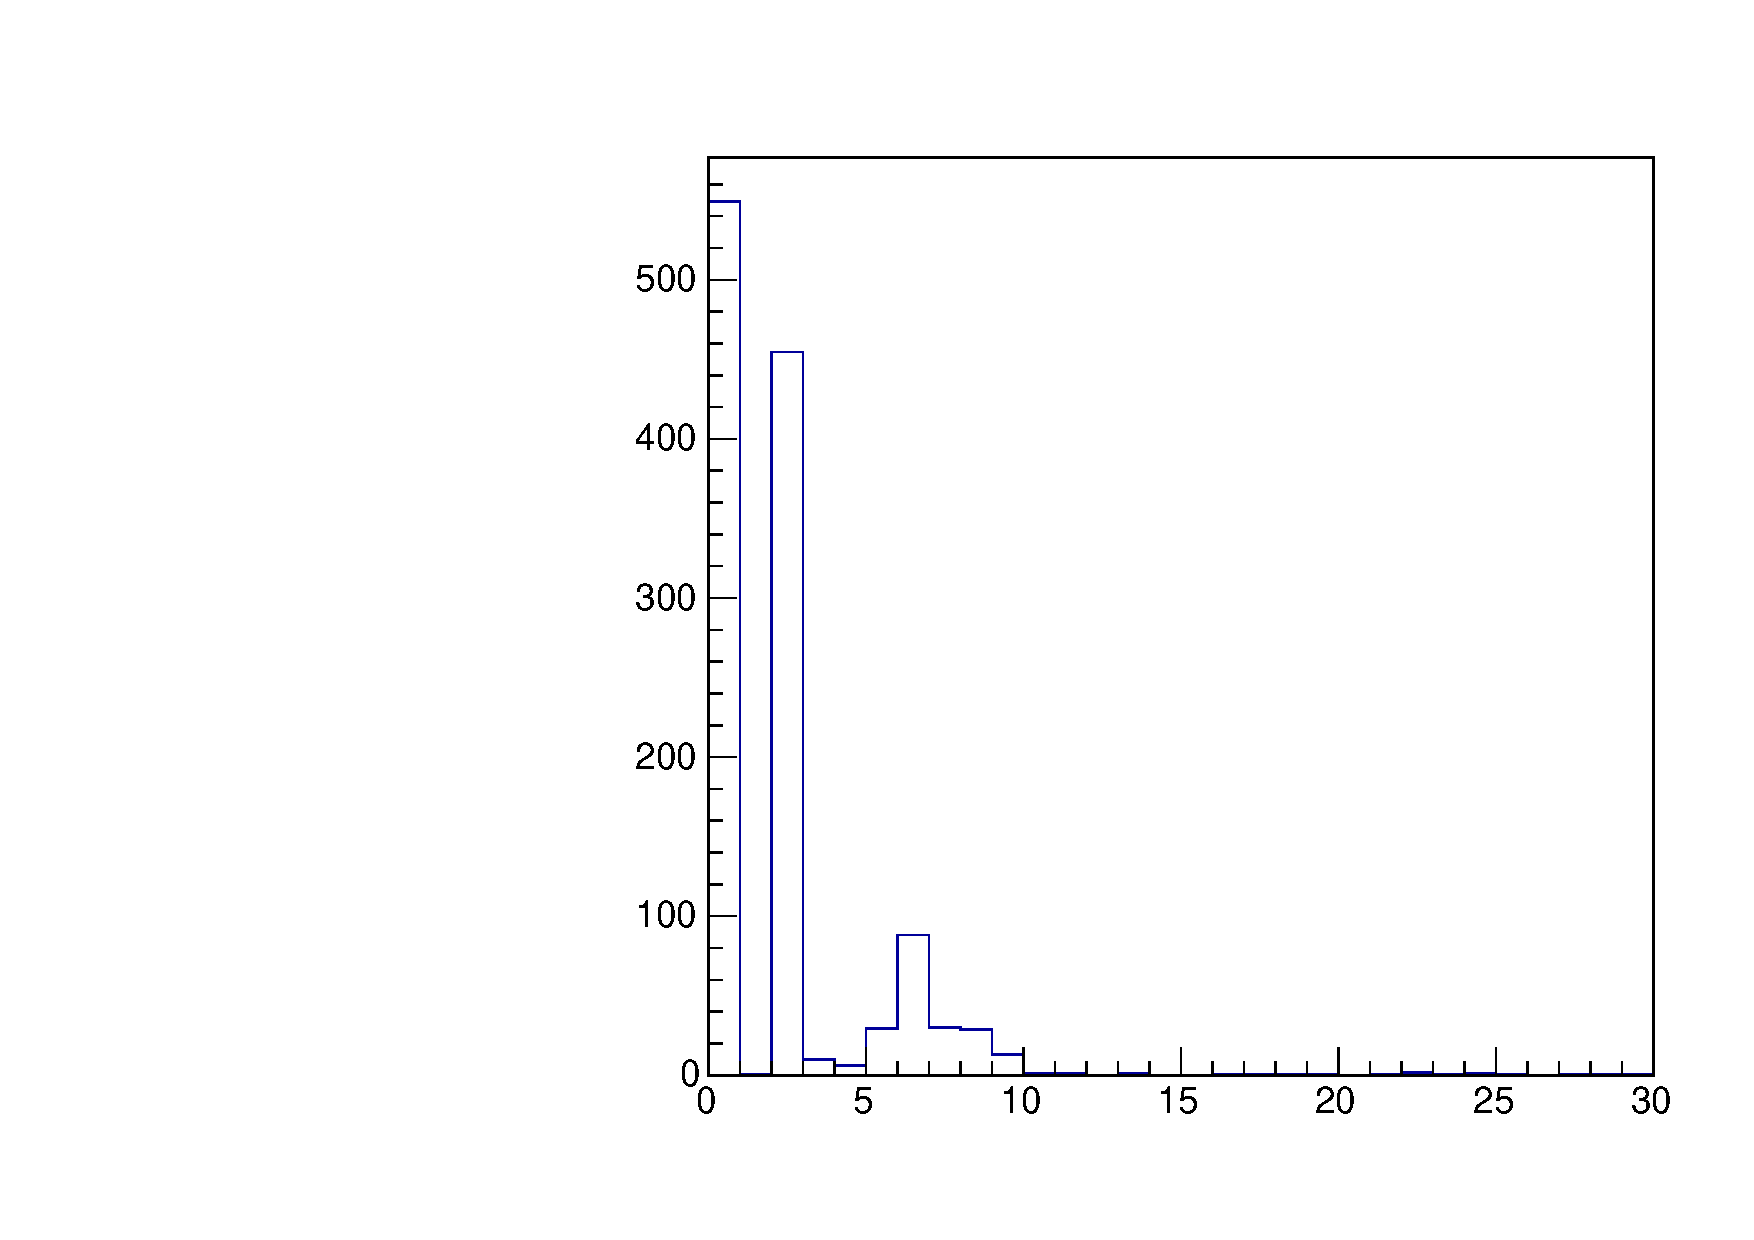
\includegraphics[width=0.49\textwidth]{figs/unfold-svd-ddistr.pdf}
	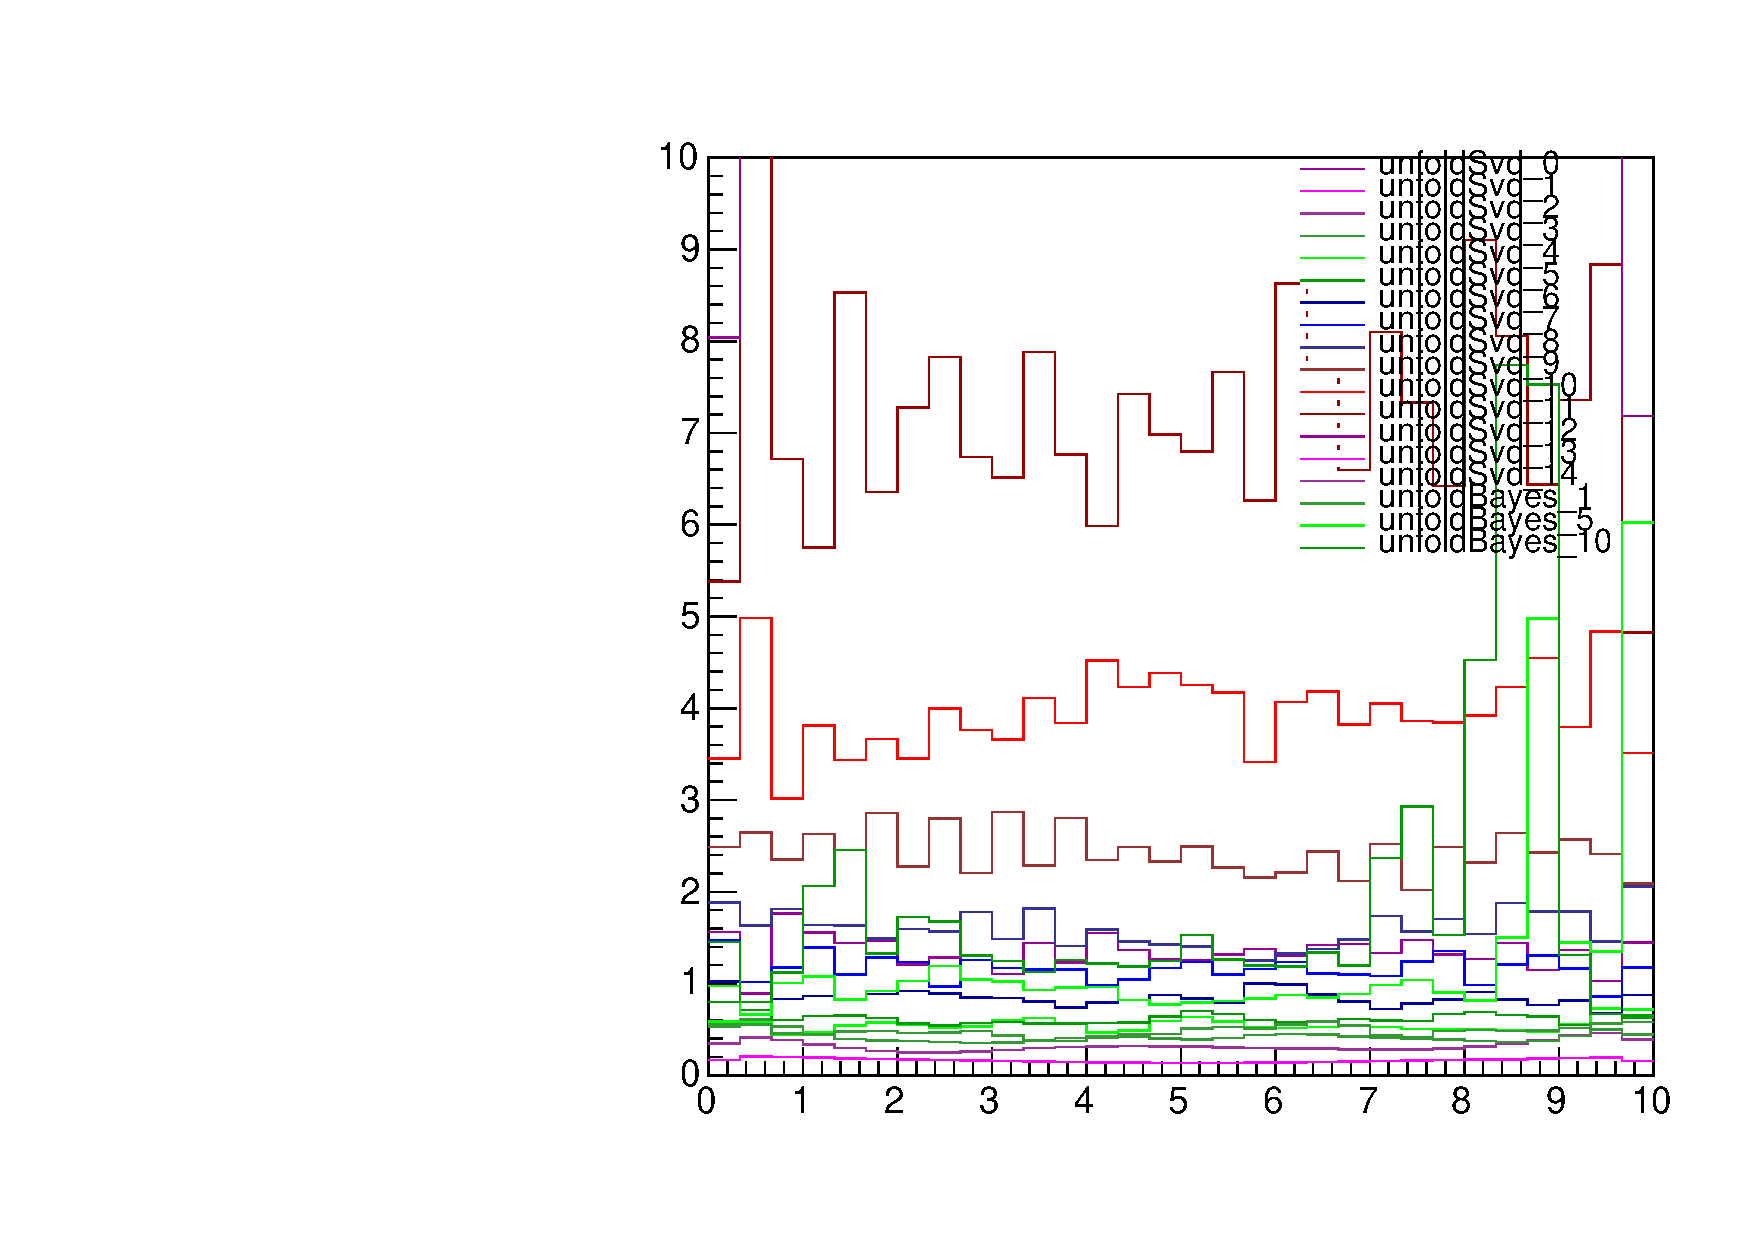
\includegraphics[width=0.49\textwidth]{figs/unfold-error-reg.pdf}
	\caption{ \label{fig:sol:reg2} Left: $d_i$-distribution for the \gls{SVD}-method. Right: ratio of the error before and after the unfolding.}
\end{figure}

The inversion method is the \gls{ML} estimator, and therefore unbiased. If the variance of this method is under control, it is probably a good method to be used. 

The \gls{SVD}-method penalizes distributions accordingly to the curvature they use, therefore it is not suited to unfold rapidly changing distributions expecially with bumps (with respect to the \gls{MC} residuals).

The iterative method will rapidly converge the \gls{ML} solution if a good starting point is used (\gls{MC}). 

Both regularized unfolding method assume a binning (which is an other way of regularize) and uses a migration spectra from the simulation, which may leave some model dependence.

\FloatBarrier
\section{Construct the response matrix}

The response matrix can be constructed in the following steps:

\begin{enumerate}
\item  Define a flag to identify if the event is in the fiducial region at the measured/truth level:
\begin{verbatim}
        isGen = t.lep1PtTruth >=15 and t.lep2PtTruth >= 15 \  
                and abs(t.lep1EtaTruth )<2.5 and abs(t.lep2EtaTruth) <2.5
        isReco = t.lep1PtReco >=15 and t.lep2PtReco >= 15  
                and abs(t.lep1EtaReco )<2.5 and abs(t.lep2EtaReco) <2.5
\end{verbatim}

\item Compute the scale factor as product of the two lepton scale factors.

\item Define the reconstructed TLorentzVector using the muon mass ($m_\mu \approx 0.105$ GeV ), and from the leptons the $Z$ ones at generator level ($Z$) and at reconstruction level ($LL$)

\item Fill the gen histogram if it is in the fiducial volume at generator level:
\begin{verbatim}
        if isGen: hTruth.Fill(Z.Pt(), t.weight ) # no sf
\end{verbatim}

\item Fill the reconstructed level with the scale factors, if it is in the fiducial volume at reconstruction level
\begin{verbatim}
        if isReco: hReco.Fill( LL.Pt(), t.weight * mysf)
\end{verbatim}

\item Fill the smearing matrix if both level are matched:
\begin{verbatim}
        if isGen and isReco:hMatrix.Fill(LL.Pt(),Z.Pt(),t.weight*mysf)
\end{verbatim}

\item Unfold the distribution, eg:
\begin{verbatim}
        R = ROOT.RooUnfoldResponse(hReco,hTruth,hMatrix)
        R.UseOverflow()
        u = ROOT.RooUnfoldBayes(R,hData,20)
\end{verbatim}
\end{enumerate}

Results can be seen in figure~\ref{fig:sol:exe2}.
A  couple of possible mistakes are also represented in fig.~\ref{fig:sol:exe2}:
the not correct application of the scale-factors will result in a generally low yield under the peak (green) because the efficiencies assumed by the unfolding are slightly wrong, while the non application of the \gls{MC}-weights (magenta) will make the unfold distribution sensitive to the way this weights are produced, that for this particular case are correlated with the $p_{T}^{Z}$ and produces spikes in the points corresponding to the changes of these weights ($p_{T}^{Z} = 10, 20, 50$ GeV). 
Finally, neglecting the overflow bins, does not allow the unfolding to correctly compute the migration in from events having $p_{T}^{Z}> 100$ GeV, resulting in a small wiggle at $100$ GeV. An other possible way to consider the last effect is to include in the background and efficiency terms ( \verb@isGen = isGen && Z.Pt() <100@, \verb@isReco = isReco &&  LL.Pt() <100@), being a little more model-dependent, since this bins are completely taken from the \gls{MC} instead of only the migrations.

\begin{figure}[H]
	\centering 
	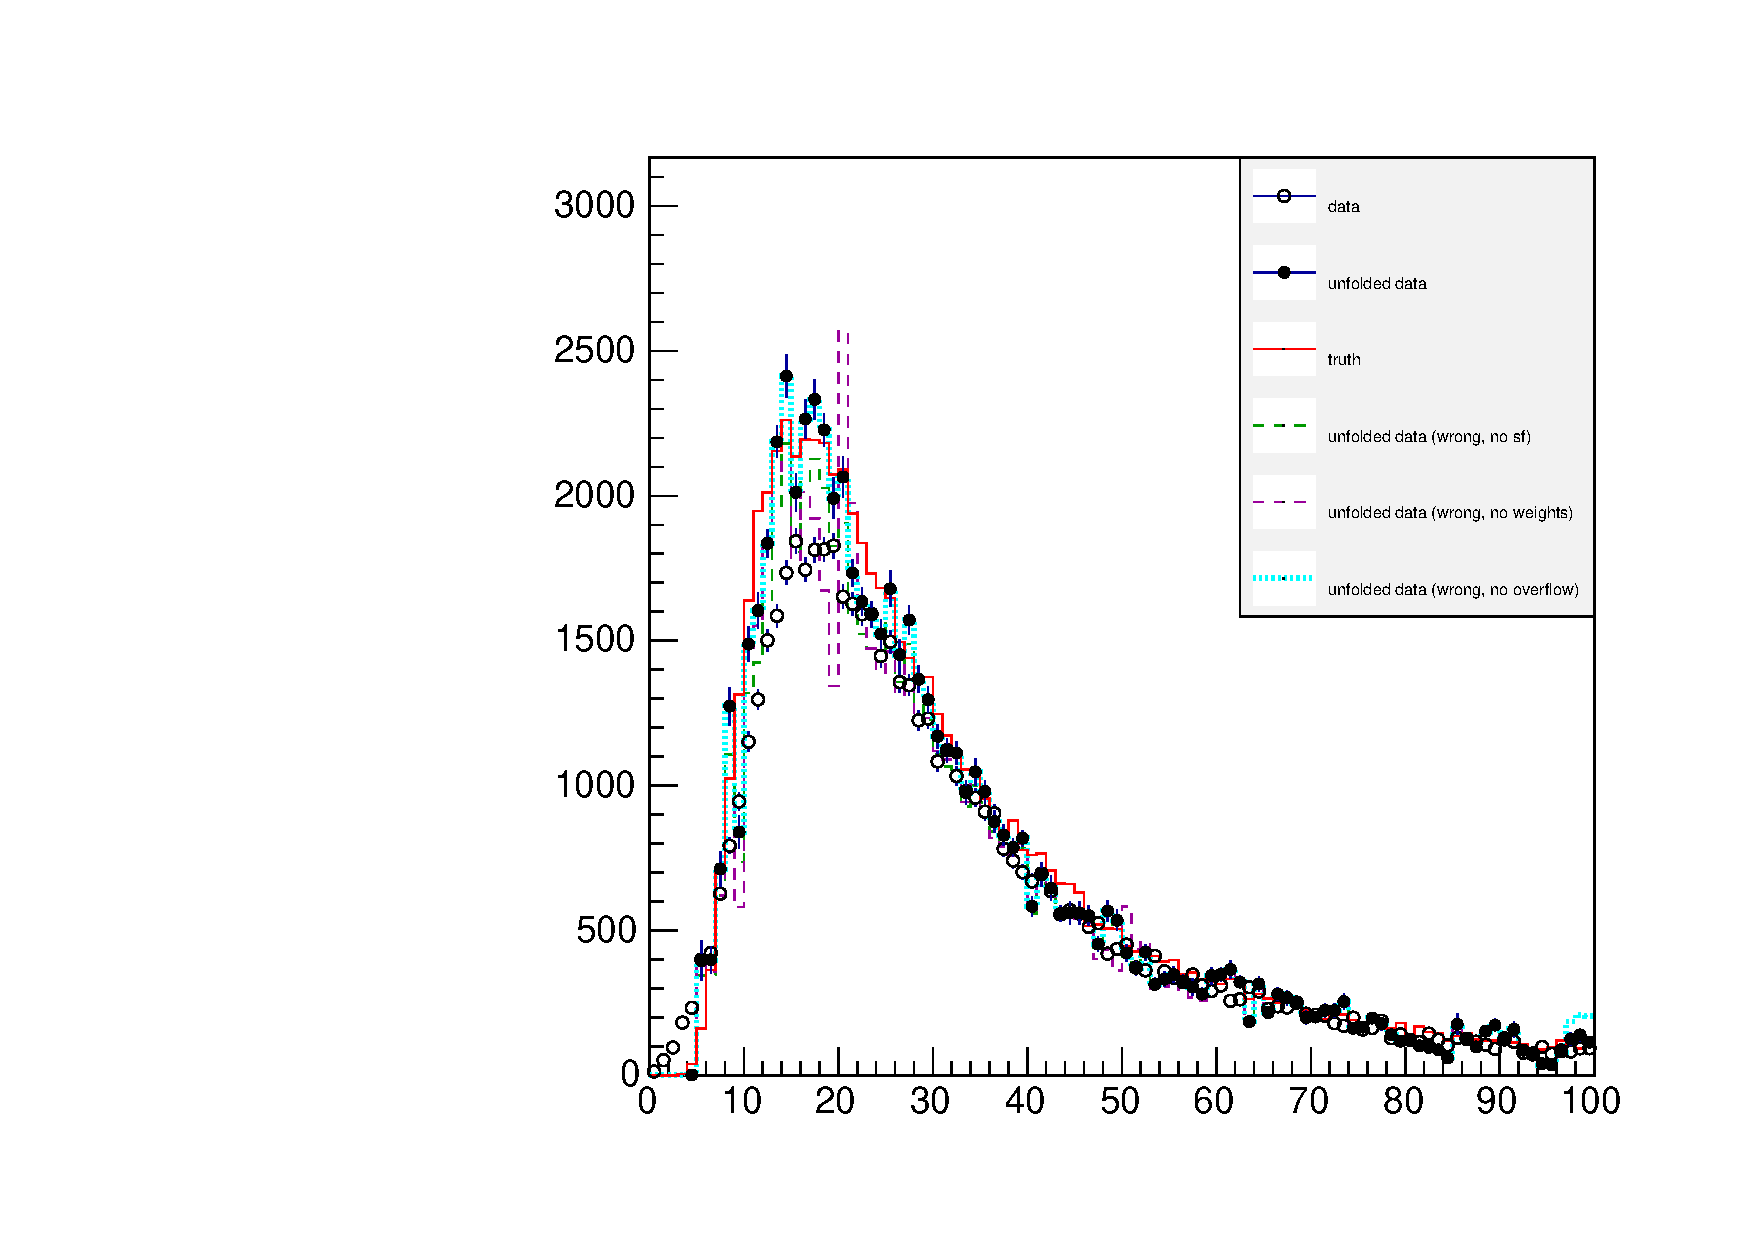
\includegraphics[width=.95\textwidth]{figs2/unfolding2.pdf}
	\caption{ \label{fig:sol:exe2} Unfolded distribution (solid black dots) compared to the reconstructed data distribution (empty dots). Underlying can be seen the distribution used to generate the data, prior Poisson fluctuations (red), and some examples of wrongly unfolded distributions (dashed): the first without applying scale-factors (green), the second considering no weights at all (magenta), and the third (cyan) without including the overflow and underflow bins.
	}
\end{figure}

The bumpy structure at $\approx70\,\textup{GeV}$ is a structure present only in the data distribution but not in the \gls{MC}-model given in the tree.
\begin{figure}[H]
	\centering
	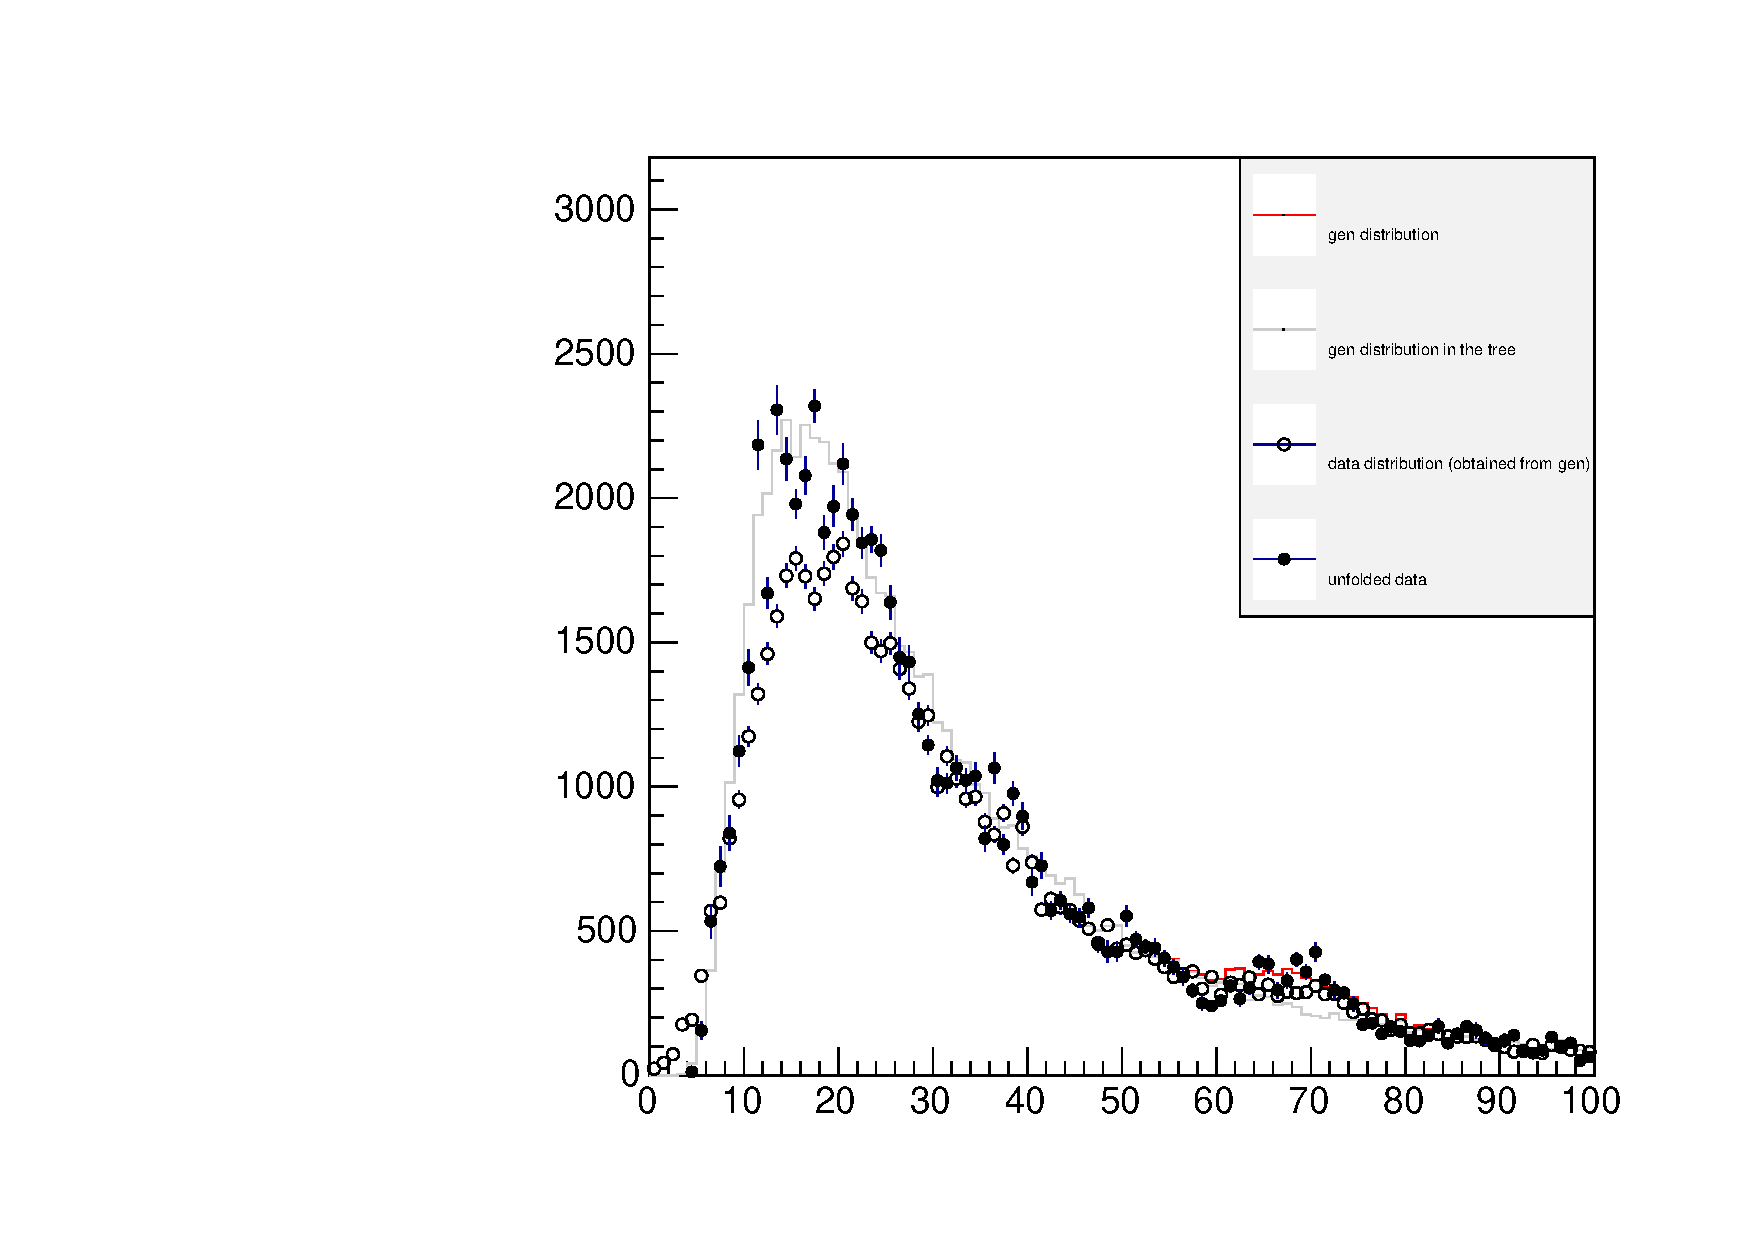
\includegraphics[width=0.49\textwidth]{figs2/bump.pdf}
	\caption{ \label{fig:sol:bump} A bump structure at $\approx 70\,\textup{GeV}$ added to the data distribution and visible in the unfolded one. The gray line represent the generated sample without such structure used for filling the \gls{MC}-simulation given in the tree.
	}
\end{figure}

The constructed unfold matrix is:
\begin{figure}[H]
	\centering
	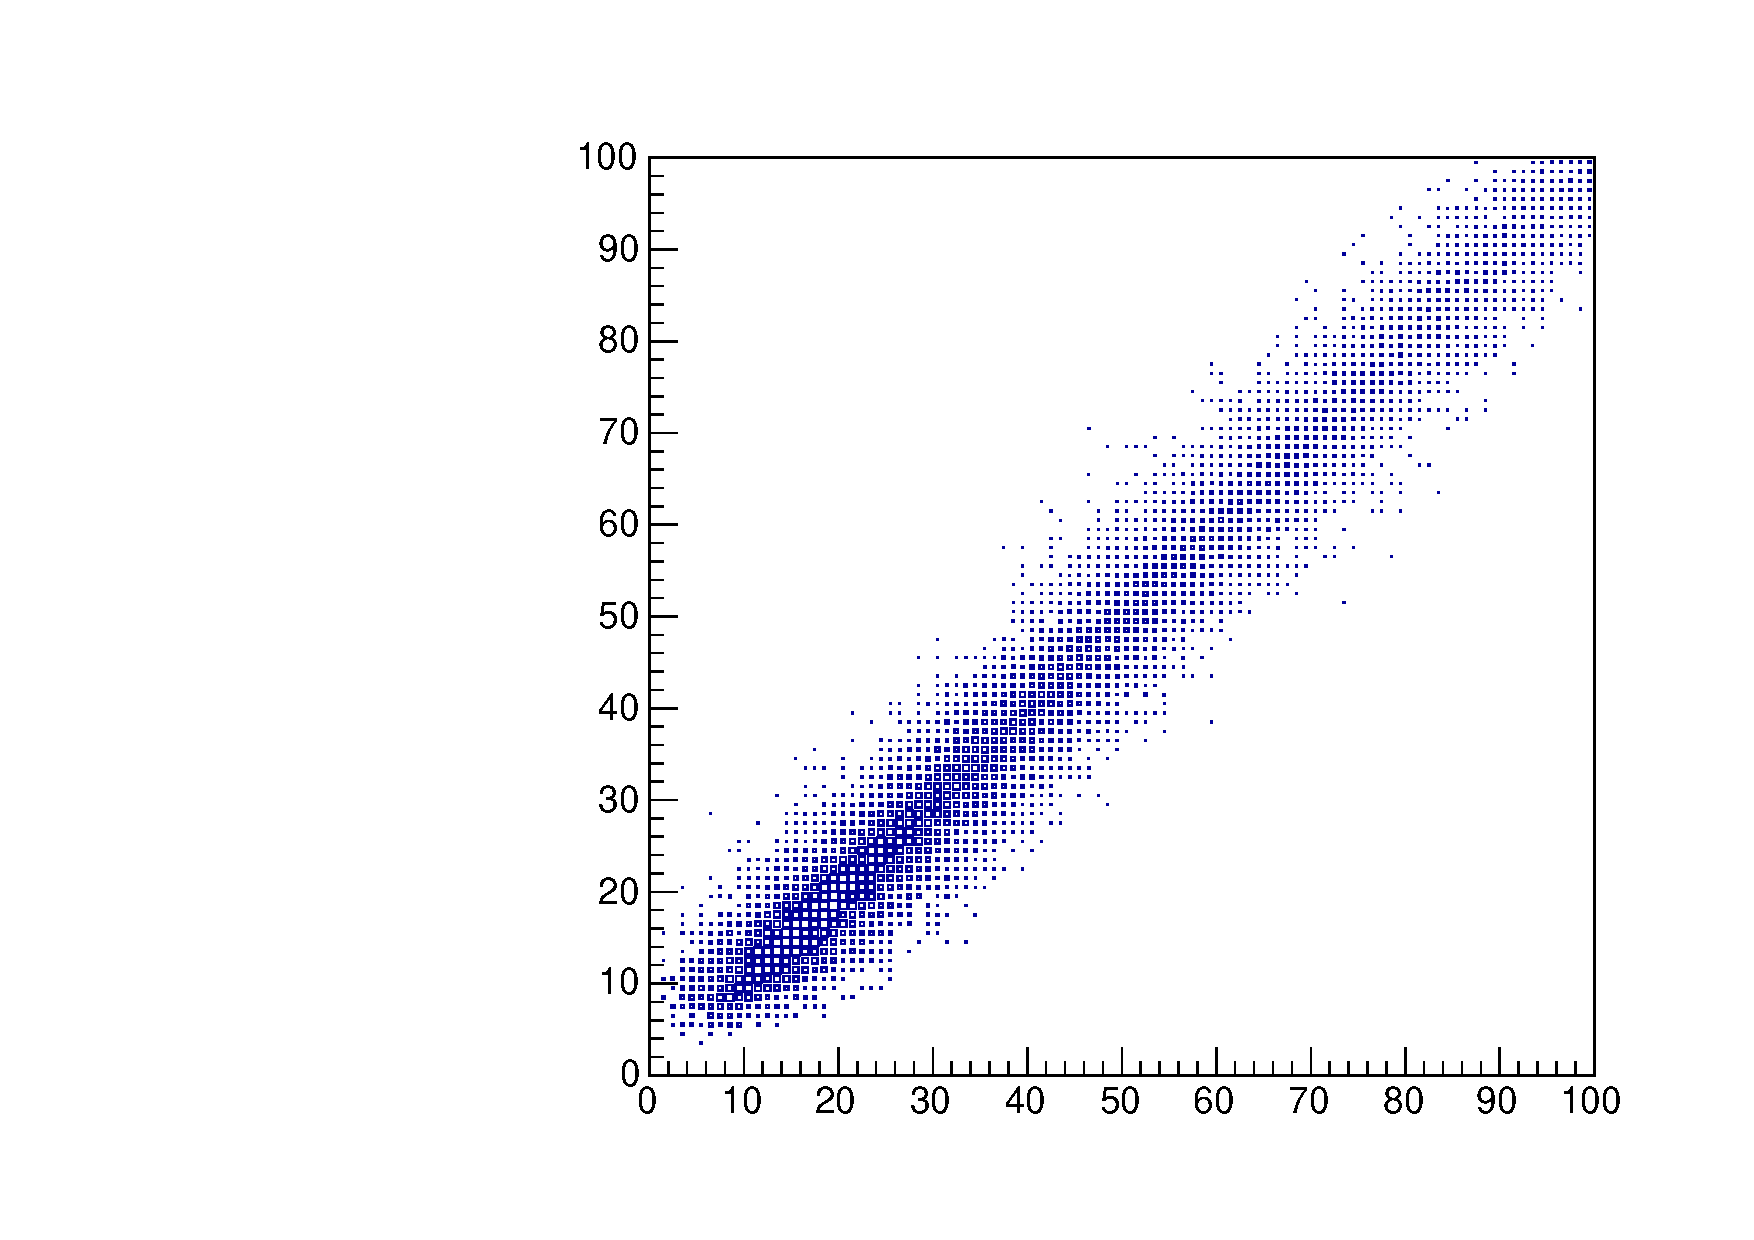
\includegraphics[width=0.49\textwidth]{figs2/matrix.pdf}
	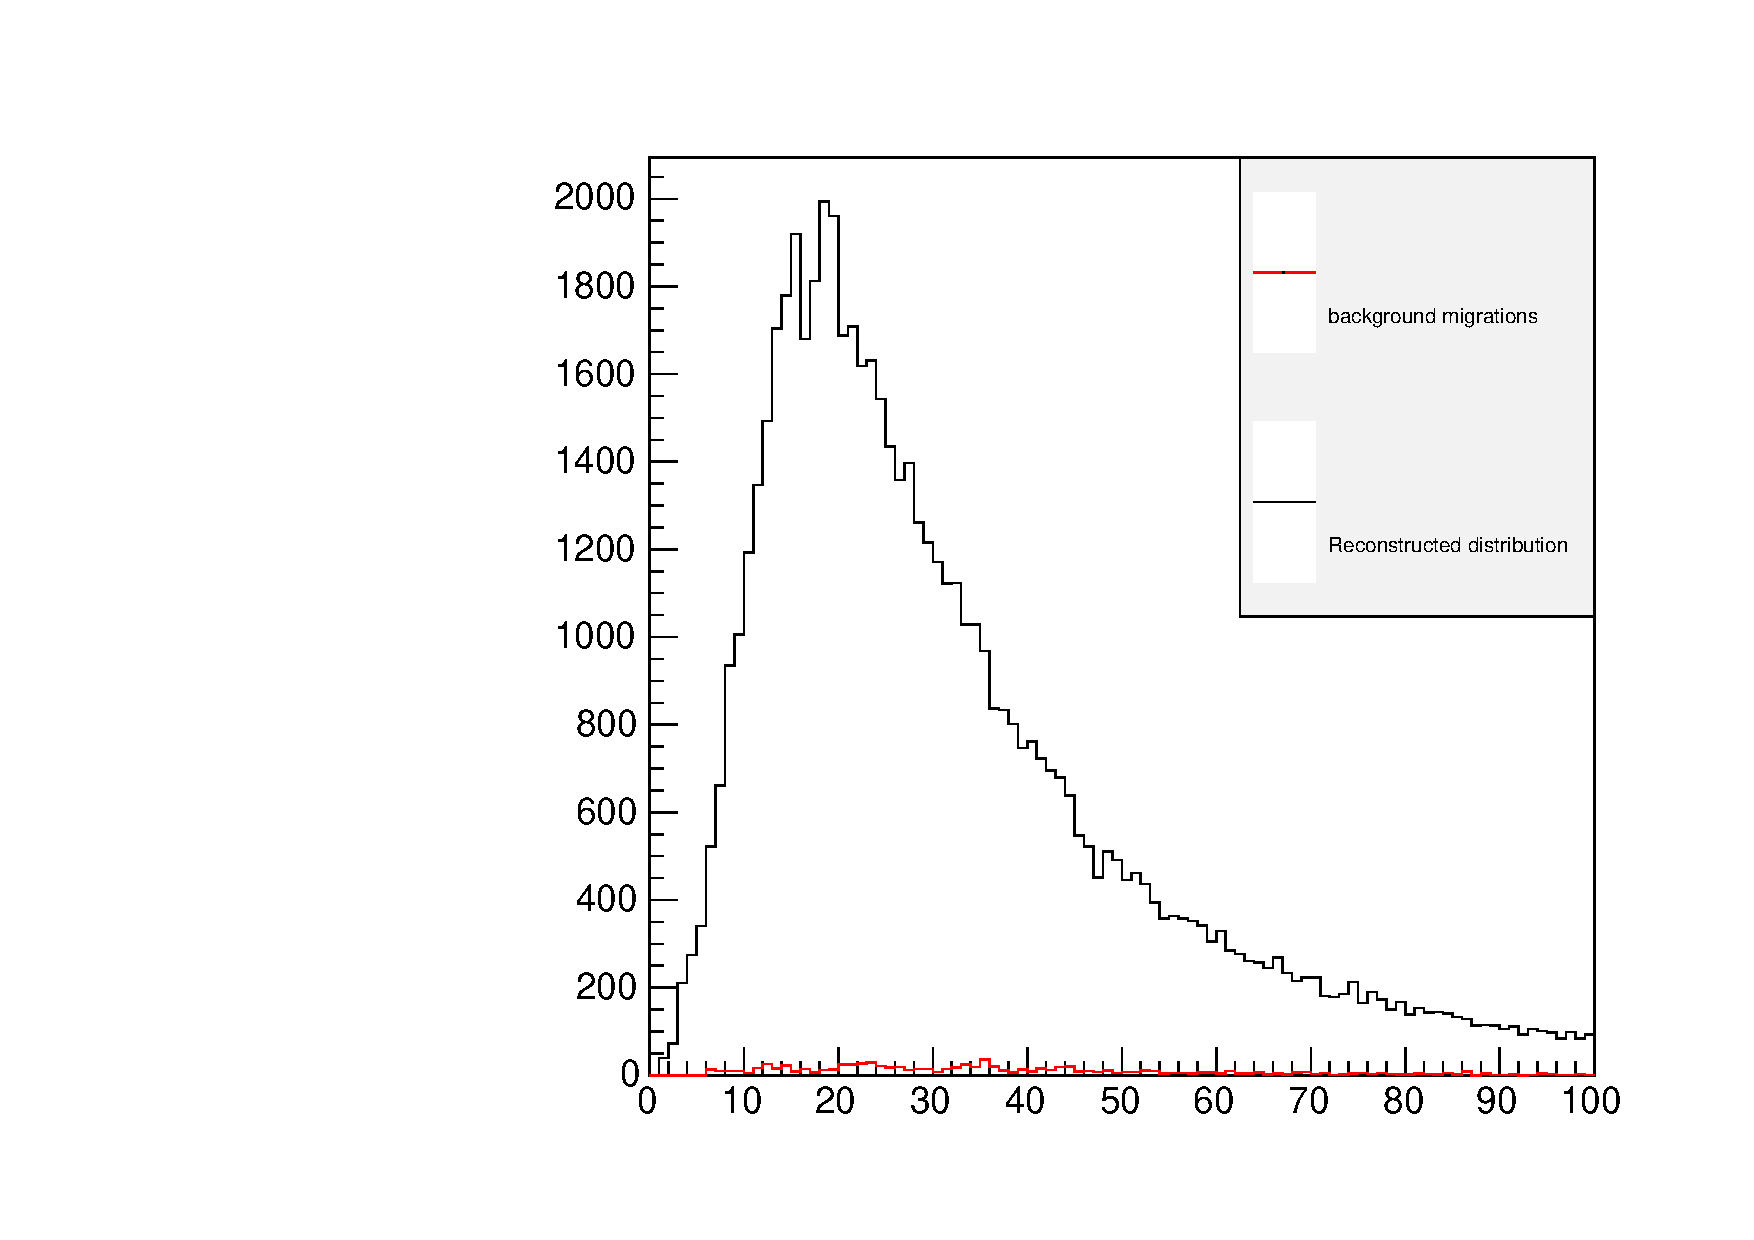
\includegraphics[width=0.49\textwidth]{figs2/bkg.pdf}
	\caption{The smearing matrix ($\mathbf{R}$) used in the unfolding (left), and the background component ($\vec{b}$) compared to the expected distribution corrected for scale factor efficiencies (right).
	}
\end{figure}

The number of events generated and recovered with a Bayesian unfolding in the two selections are:
\begin{table}[H]
\centering
\begin{tabular}{lrrr}
	\toprule 
	bin & generated & Bayes \\
	\midrule
	$[10,20)$  & $ 20877 $  & $20161$ \\
	$[98,100)$ &  $ 181 $  & $ 194 $ \\
	\bottomrule
\end{tabular}
\caption{number of events generated and reconstructed in the two selections.}
\end{table}

The absence of the correct overflow handling leads to an excess of event in the $[98,100)$ selection ($439$).
	On the other hand, a  mistake in the scale-factors ends up in a lower yield in the bins $[10,20)$ (e.g., no-scalefactor $18200$).


\end{document}
